%\documentclass[journal]{IEEEtran}
\documentclass[10pt,twocolumn,twoside,letterpaper]{IEEEtran}

\usepackage{geometry}
\geometry{letterpaper, top=0.7in, bottom=0.7in, left=0.65in, right=0.65in}

% If IEEEtran.cls has not been installed into the LaTeX system files,
% manually specify the path to it like:
% \documentclass[journal]{../sty/IEEEtran}

\makeatletter
\def\ps@IEEEtitlepagestyle{
  \def\@oddfoot{\mycopyrightnotice}
  \def\@evenfoot{}
}
\def\mycopyrightnotice{
  {\footnotesize
  \begin{minipage}{\textwidth}
  \centering
  978-1-6654-2113-3/21/\$31.00 \copyright2021 IEEE
  \end{minipage}
  }
}

\usepackage{multirow}
\usepackage{longtable}
\usepackage{graphicx}
\usepackage{subcaption}
\usepackage{url}
\usepackage{hyperref}
% correct bad hyphenation here
\hyphenation{op-tical net-works semi-conduc-tor}


\begin{document}
\title{
Deep network optimization using a Genetic algorithm for recognizing hand gestures from EMG Signal
}
\author{Kasra Sehhat, Alireza Khodabakhsh, Arman Aghaee}



% make the title area
\maketitle

\pagenumbering{gobble}


% As a general rule, do not put math, special symbols or citations
% in the abstract or keywords.
% ================================================== %
% ABSTRACT
% ================================================== %
\begin{abstract}
Hand gesture recognition has many applications in engineering and health care. This paper proposes a model that accurately distinguishes hand gestures using the surface electromyographic (sEMG) signals of forearm muscles. For this purpose, deep learning algorithm and convolutional neural network (CNN) have been used in the recognition stage. The deep neural network contains hyperparameters that affect the final accuracy of the model. In this study, The number of convolutional layers, the number of kernels per layer, and the number of dense layer’s neurons are selected for optimization, and the remaining parameters, such as the learning rate, batch size, and the number of epochs are selected based on the try and error and prior knowledge. The optimal values for selected hyperparameters are obtained using a genetic algorithm to achieve maximum recognition accuracy. The UC2018 database was used to train and test the model, including EMG signals related to 8 hand gestures. The model's structure consists of 2 convolutional layers with 131 and 28 kernels, a dense layer with 111 neurons, and finally, a softmax layer with 8 neurons. After optimizing the hyperparameters using the genetic algorithm, the proposed model's accuracy increases from 91.86\% to 96.4\% at best, and 95.3\% on average in real-time usage. The accuracy of the optimized model in offline mode is 99.6\%. The source code is available
 \url{https://github.com/AlirezaKhodabakhsh/Genetic_EMG}
\end{abstract}

% Note that keywords are not normally used for peer review papers.
\begin{IEEEkeywords}
%IEEE, IEEEtran, journal, \LaTeX, paper, template.
Gesture Recognition, sEMG, Deep Learning, Genetic Algorithm
\end{IEEEkeywords}



% ================================================== %
% INTRODUCTION
% ================================================== %
% HELP
% bold: {\bf The deadline for the submission of a manuscript to the CR is 1 December 2021.}
% \textit{IEEE Transactions on Nuclear Science (TNS)}

\section{Introduction}
\IEEEPARstart{T}{he} EMG signal directly results from the muscles' electrical activity during contraction and can be considered a means of decoding body movements [1]. Human motion detection using EMG signals, known as EMG pattern recognition, has been employed in various applications, including powered upper-limb prostheses [2], electric power wheelchairs [3], human-computer interactions [4], and diagnosis in clinical applications [5]. Compared to other well-known bioelectrical signals (e.g., electrocardiogram) ECG), the electrooculogram (EOG), and galvanic skin response (GSR)), the analysis of surface EMG signal is more challenging [6]. Some of these challenges include the changing characteristics of the signal itself over time, electrode location shift, muscle fatigue, variations in muscle contraction intensity, limb position changes, and forearm orientation. However, due to its non-invasive nature and ease of recording sEMG signals, its use is superior to other methods [7-12].

The most common EMG pattern recognition algorithms include support vector machine (SVM), K nearest neighbor (K-NN), Linear discriminant analysis (LDA), multilayer perceptron (MLP), artificial neural network (ANN), and random forest classifiers. Ahmad Alkan and Mucahid Gunay [14] have claimed that they could classify four EMG data classes with 97±1\% accuracy using the SVM algorithm. Tkach et al. [15] used the LDA algorithm to classify the data. They achieved 92\% accuracy for 13 classes. Z. Li et al. [16], using a boosted random forest classifier, achieved a RR of 92\%, but the novelty detection accuracy was 20\%. The authors tuned the algorithm so that there is a novel detection accuracy of 80\%, but the RR in trained samples decreased to 80\%. In the mentioned methods, the step before classification is feature extraction, which is done manually.

Although feature engineering has been the dominant focus for EMG pattern recognition so far, feature learning, as exemplified by deep learning, has recently started to demonstrate better recognition performance than hand-crafted features. Unlike feature engineering and conventional machine learning approaches, deep learning can take advantage of the multiplicity of many samples to extract high-level features from low-level inputs. However, deep learning algorithms require large training datasets to train large deep networks (a few hidden layers, each with a large number of neurons) and an associated large number of parameters (millions of free parameters). Nowadays, despite large datasets and advances in processing technology, deep learning algorithms in EMG pattern recognition are less restricted [17].

Geng et al. [18] evaluated CNN's performance in recognizing hand and finger motions based on sEMG from three public databases containing data recorded from either a single row of electrodes or a 2D high-density electrode array. Without using windowed features, the classification accuracy of an eight-motion within-subject problem achieved 89.3\% on a single frame (1 ms) of an sEMG image and reached 99.0\% and 99.5\% using 128 channels HD-sEMG signals and simple majority voting over 40 and 150 frames (40 and 150 ms), respectively. Côté-Allard et al. [19,20] showed that CNN is accurate enough to detect complex movements. It is also robust to short-term muscle fatigue, small displacement of electrodes, and long-term use without recalibration. Laezza [21] evaluated three different network models' performance, including RNN, CNN, and RNN + CNN for myoelectric control. Based on their work, RNN provided the best performance with 91.81\%  classification accuracy compared to CNN (89.01\%) and RNN + CNN (90.4\%). This result may be due to RNN and LSTM networks' advantages in time series processing. Ali Raza Asif et al. [22] investigated the effect of hyperparameters on each hand gesture. They showed that the learning rate set to either 0.0001 or 0.001 significantly outperformed other considerations.

In the present study, the UC2018 database [23] has been used to train a deep convolutional neural network. Since the dataset does not have enough data for deep network training, more data has been generated using the windowing technique [24]. First, the basic model, a deep convolutional network, is trained by the data obtained. Due to a large number of variables, the initial model does not necessarily have the maximum accuracy. Therefore, to achieve maximum accuracy, the model structure is optimized by a genetic algorithm [25]. Finally, the model confusion matrix is proposed using the optimal parameters, representing the designed model's performance.



% ================================================== %
% PRE-PROCESSING
% ================================================== %
\section{Preprocessing}
At this stage, the EMG signals should be recorded by the armband and the hand movements by the data glove to create a database containing the type of gestures and the corresponding signal.  Recorded signals are raw data and require preprocessing to be used for network training and testing. The preprocessing phase includes filtering, normalizing, windowing, labeling the data, and finally converting it into three subsets: train, validation, and test [26,27].

The UC2018 database is used to avoid prolonging the research path. This data set is obtained from two EMG sensors (Myo) with a subject that performs eight distinct hand gestures. There are a total of 110 repetitions of each class of gesture obtained across five recording sessions. Each armband contains eight sensors that record data at a frequency of 200 Hz. Since the sampling time is 2 seconds, the dimension of the data is 16×400. Some preprocessing steps have been performed in this database, including removing municipal electricity and heartbeat noise [28]. Figure 1 shows eight movements related to the signals of this database.

\begin{figure}
    \centering
    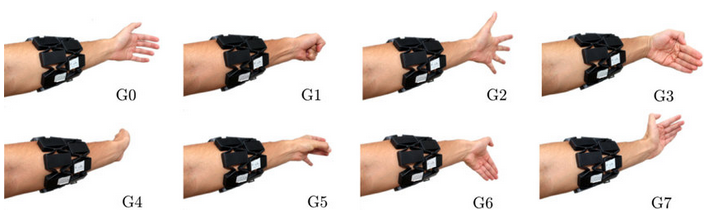
\includegraphics[scale=0.49]{figures/gestures.png}
    \caption{\centering
    UC2018 DualMyo dataset gestures: (G0) rest, (G1) closed fist, (G2) open hand, (G3) wave in, (G4) wave out, (G5) double-tap, (G6) hand down, (G7) hand up}
    \label{fig:gestures}
\end{figure}

Although the noise removal operation performed on the data set, the data is still not suitable for model input. The signals are long, and the amount of data to train the deep network is not sufficient. In order to solve this problem, first, the signals are stacked, and then using the windowing technique data is split into signals with less length. For this purpose, the length of each window and the amount of overlap must be specified. In this study, the window size is 125 milliseconds for real-time and 1 second for offline usage without overlap. The last 15 and 50 data of each sample is used for labeling, respectively, and the label with the most repetition is selected as the sample label. 14080 signals with dimensions of $25 \times 16$ and $200 \times 16$ were obtained, which are both the right size and sufficient number. The signal range is -128 to 128. In order to increase the speed of convergence of the network and also stabilize the network and preventing from gradient exploding, it is necessary to normalize the input data. For this reason, the MinMax is used and all data are divided by the maximum value, 128 so that the data are in the range of -1 and +1. The data were then randomly divided into three train, test, and validation groups, with a ratio of 70\%, 15\%, and 15\%  so that the test data is completely unseen.

% ================================================== %
% MODEL-DESIGN
% ================================================== %
\section{Model Design}
This part of the research is the most important because the structure of the model and the model's parameters significantly impact the accuracy of hand gesture recognition. The choice of model depends on the dimensions and number of data as well as their nature. However, choosing model parameters requires trial and error, making the design process complicated and time-consuming [29]. The number of model parameters can also be one of the design variables, but this study's primary purpose is to maximize the model's accuracy in pattern recognition. 

Input data are labeled, so the present model is a supervised model. In traditional machine learning and classification methods, the model requires a section that extracts a series of features from the input signals. The classifier then divides the signals into different classes based on these features. The accuracy of these models strongly depends on the selected features. The deep CNN network, selected as the present classifier model, extracts high-level data features by convolutional layers. This feature extraction method, called feature learning, performs better than traditional hand-crafted features[30].

The model consists of a series of convolutional layers, a dense layer, and a SoftMax layer with eight neurons [31]. Each convolutional layer contains kernels of specified dimensions. These kernels move on the signal with a fixed step and extract the properties. In this research, rectified linear units (Relu) have been used as an activation function to prevent the Gradient vanishing phenomenon and improve the training speed [32]. The dimension of the kernels are 20 × 8, and their step size is one. The number of convolutional layers, the number of neurons of dense layer neurons, and  The number of kernels in each layer are the parameters whose optimal value will be calculated using the genetic algorithm. The last layer of this model consists of 8 neurons with the SoftMax activation function. 

A high value of the learning rate causes training to fluctuate and may not to be converged , and a low value reduces the convergence rate of the model. The learning rate choice also affects the number of epochs; the lower the learning rate, the higher the epochs. On the other hand, a high number of epochs may overfit the model [33]. Figure 2 shows that with a higher learning rate, the model converges faster, but at higher epochs, overfitting occurs. On the other hand, model training with a small learning rate requires higher processing power. According to the experimental results, the number of epochs is 30, the learning rate is 0.0001, and the Batch size is 65. Also, the activation functions and the kernel size in all layers are relu and 20 × 8.  These parameters can also be added to independent variables optimized by the genetic algorithm, but with each parameter's addition, the computation time will increase. Therefore, in this study, only the model structure parameters, including the number of convolutional layers, the number of kernels in each layer, and the number of dense layer's neurons, are considered independent variables. In this model, the Adaptive moment estimation optimizer is used to train the coefficients, the categorical cross-entropy is used as the error function, and The coefficients are initialized by the random uniform method [34,35].


\begin{figure}
    \centering
    \begin{subfigure}[b]{0.2\textwidth}
        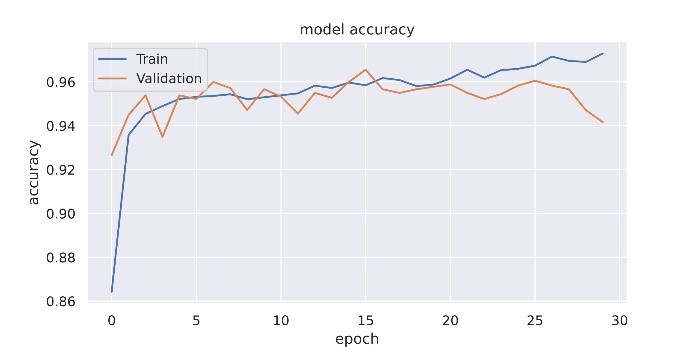
\includegraphics[width=\textwidth]{figures/lr/1.jpg}
    \end{subfigure}
    \begin{subfigure}[b]{0.2\textwidth}
        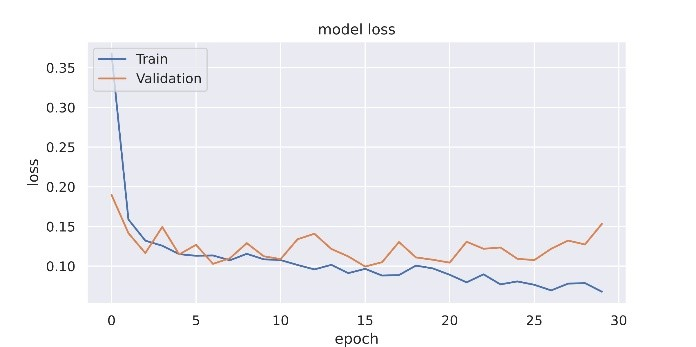
\includegraphics[width=\textwidth]{figures/lr/2.jpg}
    \end{subfigure}



    \begin{subfigure}[b]{0.2\textwidth}
        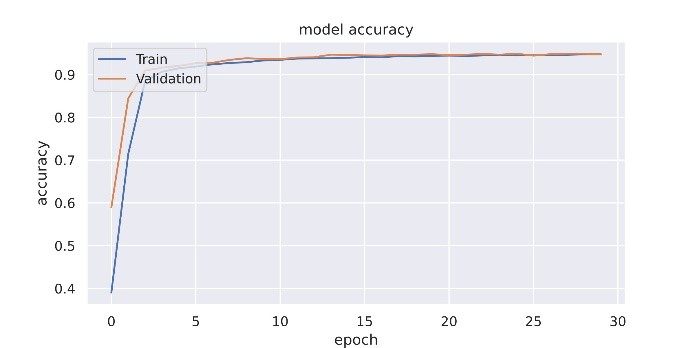
\includegraphics[width=\textwidth]{figures/lr/3.jpg}
    \end{subfigure}
    \begin{subfigure}[b]{0.2\textwidth}
        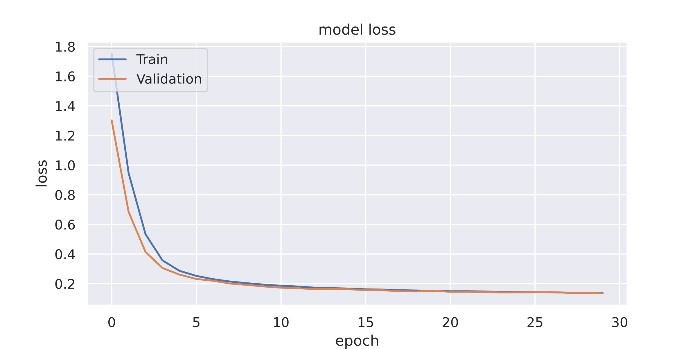
\includegraphics[width=\textwidth]{figures/lr/4.jpg}
    \end{subfigure}
    \caption{\centering
    Comparison of model accuracy and loss  for learning rate 0.0001 (top) and 0.00001 (bottom}
    \label{fig:lr_s}
\end{figure}

% ================================================== %
% MODEL- OPTIMIZATION
% ================================================== %
\section{Model Optimization}
In the previous section, a model was used to recognize hand gesture based on the EMG signal. However, this model includes parameters that a slight change in each affects the accuracy of the model. Therefore, it is essential to select these parameters so that the model is most accurate. So we are faced with an optimization problem, and the cost function is the accuracy of the convolutional model in detecting hand gesture. One way to get the optimal answer is to experiment with different structure of models and choose the best answer. However, this is time-consuming, and a limited number of models can be tested. The optimal answer obtained in this way is probably a local minimum point and not the best. A genetic algorithm is a Stochastic optimization method and uses random elements, so it is improbable to be trapped at local minimum points. As the rate of random parameters increases, this probability decreases.

The genetic algorithm determines the first generation with a specific population size so that each of the chromosomes of this generation is a structure for the convolutional model. The convolutional model is based on chromosomes' structure and provides recogntion accuracy, which is the algorithm's objective function. The chromosomes are then randomly integrated to form the next generation. The higher the chromosome score from the objective function, the better the chance of advancing to the next generation. Chromosome integration is done by cross over, mutation, parents portion, and elite portion methods [36]. This process continues until the algorithm converges and reaches the best generation. The best chromosome of this generation is selected as the optimal structure of the model.

The genetic algorithm has parameters that must be adjusted for better results. One of these parameters is the number of chromosomes in each generation, between 2 and 4 times the number of problem variables. In this case, the number of variables is 4, but for a better result, chromosomes' population is considered to be 25. The maximum number of generation sequences is a large number selected not to cause the algorithm to stop before convergence. In the crossover method, two members of the current population are randomly selected with different weight coefficients. The cross over probability coefficient is 0.7 and is selected as uniform. Each member of the new generation will be generated with a 20\% chance of crossing over. The mutation probability coefficient in this study is 0.1. The larger this number, the less likely the algorithm be trapped in a local minimum. In the parent's portion method, some parents are passed on to the next generation randomly but with different weight coefficients. The probability of choosing parents is based on the score they have earned from the objective function. The parent's portion coefficient is 0.2.  In the elite method, some elites of each generation are passed on to future generations. The share of elites from each generation is 0.05. A stop criterion is also defined to stop if the algorithm converges before reaching max iteration. If there is no increase in the objective function in 6 consecutive generations, it means that it has reached the convergence point.

The objective function of the genetic algorithm is the accuracy of the model. Therefore, for each generation member, the model must be trained, and the accuracy of the model must be determined, which makes the computational cost very high. A method has been used to reduce the computational cost as much as possible. A filter is placed in the objective function whose job is to detect duplicate inputs. If the input is duplicated and the model has already been trained with the same structure, the algorithm searches for the corresponding answer among the previous answers and records it as the objective function's output.


The research algorithm is written in Python programming language on the Tensorflow framework and the Keras library. The test runs on a computer with a 3.2GHz CPU, 32GB RAM \&  NVIDIA GeForce GTX 1080 specifications.


% ================================================== %
% RESULTS
% ================================================== %
\section{results}

The objective function of the genetic algorithm is the accuracy of the model. Therefore, for each generation member, the model must be trained, and the accuracy of the model must be determined, which makes the computational cost very high. A method has been used to reduce the computational cost as much as possible. A filter is placed in the objective function whose job is to detect duplicate inputs. If the input is duplicated and the model has already been trained with the same structure, the algorithm searches for the corresponding answer among the previous answers and records it as the objective function's output.
The research algorithm is written in Python programming language on the Tensorflow framework and the Keras library. The test runs on a computer with a 3.2GHz CPU, 32GB RAM \&  NVIDIA GeForce GTX 1080 specifications.

% ------------------------------------------------------ %
%% Please add the following required packages to your document preamble:
% \usepackage{multirow}
% \usepackage{longtable}
% Note: It may be necessary to compile the document several times to get a multi-page table to line up properly

\begin{longtable}{cccccccccc}
\caption{confusion matrix of the original model}
\label{tab:my-table}\\
\cline{2-10}
                        & \multicolumn{9}{c}{Predicted}                      \\ \cline{2-10} 
\endfirsthead
%
\endhead
%
                        &    & G0  & G1  & G2  & G3  & G4  & G5  & G6  & G7  \\ \hline
\multirow{8}{*}{Actual} & G0 & 260 & 0   & 0   & 0   & 0   & 0   & 0   & 0   \\ \cline{2-2}
                        & G1 & 0   & 251 & 0   & 1   & 0   & 0   & 0   & 0   \\ \cline{2-2}
                        & G2 & 0   & 0   & 255 & 1   & 16  & 0   & 16  & 1   \\ \cline{2-2}
                        & G3 & 0   & 0   & 0   & 256 & 0   & 4   & 1   & 1   \\ \cline{2-2}
                        & G4 & 1   & 0   & 1   & 0   & 248 & 1   & 1   & 1   \\ \cline{2-2}
                        & G5 & 82  & 0   & 1   & 1   & 0   & 160 & 0   & 14  \\ \cline{2-2}
                        & G6 & 1   & 1   & 4   & 1   & 0   & 0   & 261 & 0   \\ \cline{2-2}
                        & G7 & 0   & 0   & 2   & 0   & 0   & 7   & 0   & 251 \\ \hline
\end{longtable}

% ------------------------------------------------------ %

Table 2 shows the confusion matrix of the original model in epoch 30. The structure of this model consists of two convolutional and a dense layer. The first convolutional layer has 16 kernels, the second layer has 32 kernels, and the dense layer has 70 neurons. This structure contains 553166 independent parameters. The accuracy of this model in detecting hand movements is 91.86\%.

Table 3 shows the Precision, and sensitivity of the model for each movement. Tables 2 and 3 show that although the model successfully detected most movements, it was difficult for the model to distinguish the G0 and G5 movements. As a result, the G5's detection Precision is low, and the model's sensitivity to G0 and G5 movements is not favorable.

% ------------------------------------------------------ %
%% Please add the following required packages to your document preamble:
% \usepackage{longtable}
% Note: It may be necessary to compile the document several times to get a multi-page table to line up properly
\begin{longtable}{ccc}
\caption{Precision, sensitivity of each movement in the original model}
\label{tab:my-table}\\
\hline
   & Precision & Sensitivity \\ \hline
\endfirsthead
%
\endhead
%
G0 & 99.6      & 75.5        \\ \cline{1-1}
G1 & 99.6      & 99.6        \\ \cline{1-1}
G2 & 88.2      & 96.9        \\ \cline{1-1}
G3 & 97.7      & 98.4        \\ \cline{1-1}
G4 & 98.0      & 93.9        \\ \cline{1-1}
G5 & 62.0      & 86.9        \\ \cline{1-1}
G6 & 97.3      & 93.5        \\ \cline{1-1}
G7 & 96.5      & 93.6        \\ \hline
\end{longtable}
% ------------------------------------------------------ %

Figures 3 and 4 show the model loss and accuracy in terms of epoch for test and training data, respectively. According to these diagrams, the original model has converged, and no overfit has occurred. It can be seen that the accuracy and error of the model are fixed in the test data, and there is little fluctuation. Also, since the curve's slope is related to the test data's accuracy and error is close to zero, the model's accuracy will not change significantly as the epoch increases. Therefore, 30 epochs seem to be appropriate to achieve convergence. The number of epochs is linearly related to the time required to calculate the optimal model. However, to ensure optimal model convergence, the number of epochs varies between 10 and 100.


Using a genetic algorithm and considering the fixed parameters mentioned earlier, the model eventually converges to an optimal structure. This structure consists of two convolutional layers with 131 and 28 kernels and a dense layer with 111 neurons and a softmax layer with eight neurons. The genetic algorithm converged on this structure after 10 generations, and the time it took to use the system described in the previous section was about 34 hours and 42 minutes. To be sure, the solution was repeated 5 times. The results reported in the paper are related to the best result.

After achieving the optimal structure, the number of epochs has been changed to achieve maximum accuracy. Figures 5 and 6 show the optimal model's loss and accuracy in terms of the epoch, respectively. It can be seen that in epoch 30, the optimal model has reached convergence. As the number of epochs increases, the model's accuracy may improve slightly, but the model may become overfit.

Tables 4 and 5 show the confusion matrix and the precision, and sensitivity parameters for each movement, respectively. It can be seen that the accuracy of the model has increased after optimization and the model distinguishes G0 and G5 movements better. Since the deep learning algorithm is a stochastic method, its accuracy may vary in different runs. The accuracy of the optimal model in detecting hand movements is 96.4, and the average accuracy in 5 runs is 95\%. This indicates that the optimization has improved the deep network and the results are reliable. The model had the best performance in G1 motion detection and the weakest performance in G0 and G5 motion detection. The model's weakness in the separation of G0 and G5 is due to the hand's resting position's similarity when it is kept open.

For offline use, the window size was increased to 1 second, and a new dataset was obtained. The deep network with parameters optimized by the genetic algorithm was retrained with the new dataset. According to Figures 7 and 8, which show the loss and accuracy of this deep network, respectively, it is clear that increasing the signal length has a significant effect on the accuracy of classification. Classification accuracy in offline mode has reached 99.6\%. 

The offline network confusion matrix shown in Table 6 shows that increasing the signal length has made it easier for the network to distinguish between the G0 and G5 gestures. Although the accuracy and robustness of the model improve with increasing signal length, the larger window means more latency, making the model unsuitable for real-time use.



\begin{figure}
    \centering
    \begin{subfigure}[b]{0.2\textwidth}
        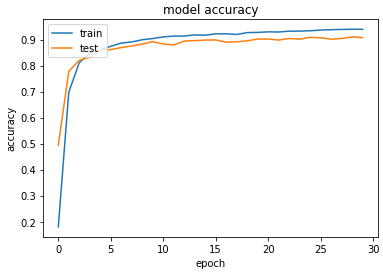
\includegraphics[width=\textwidth]{figures/Original/acc.png}
    \end{subfigure}
    \begin{subfigure}[b]{0.2\textwidth}
        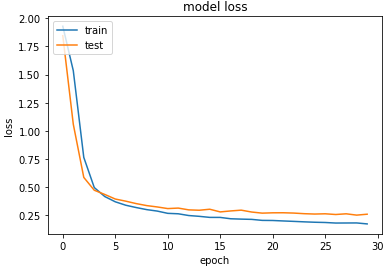
\includegraphics[width=\textwidth]{figures/Original/loss.png}
    \end{subfigure}
    
    \caption{\centering
    original models loss/accuracy in each epoch
    }
    \label{fig:original}
\end{figure}





\begin{figure}
    \centering
    \begin{subfigure}[b]{0.2\textwidth}
        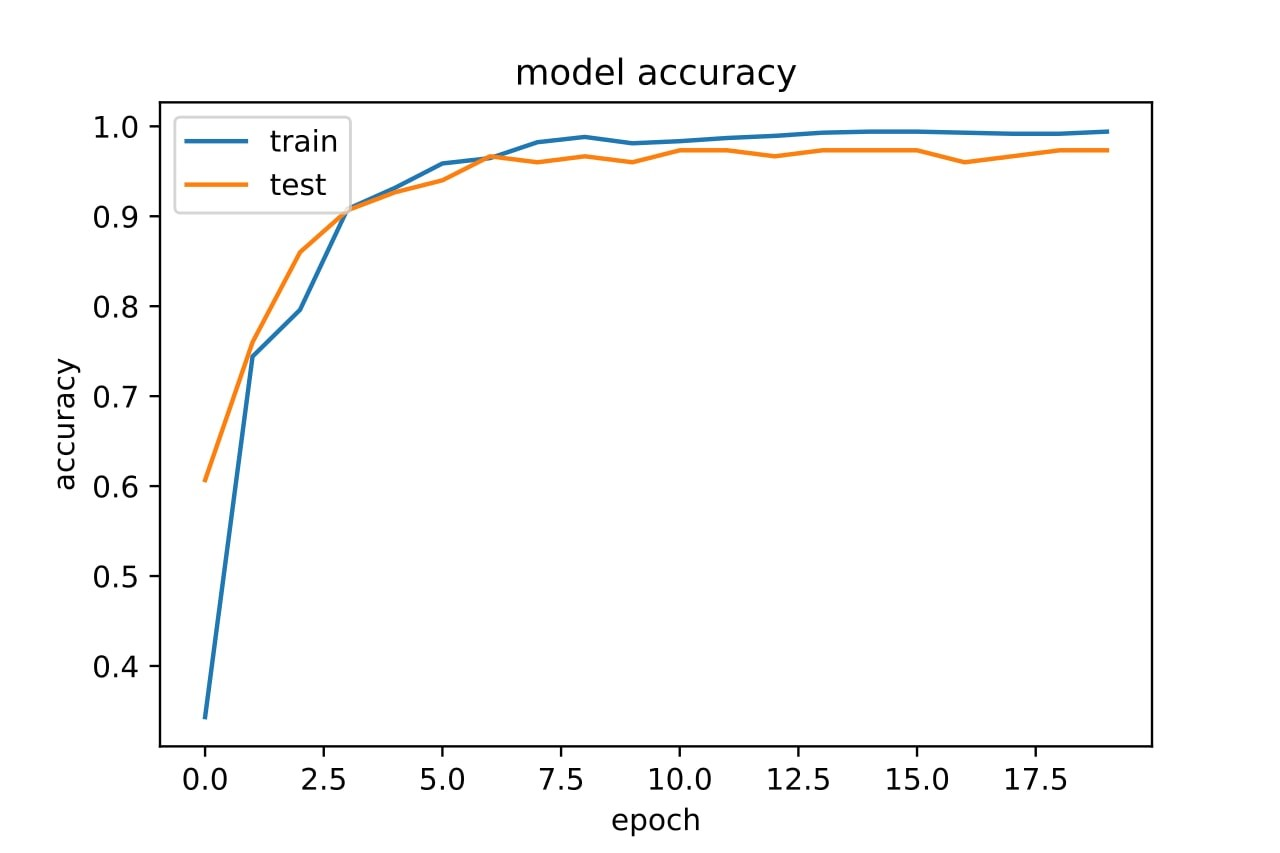
\includegraphics[width=\textwidth]{figures/Opt_RT/acc.jpg}
    \end{subfigure}
    \begin{subfigure}[b]{0.2\textwidth}
        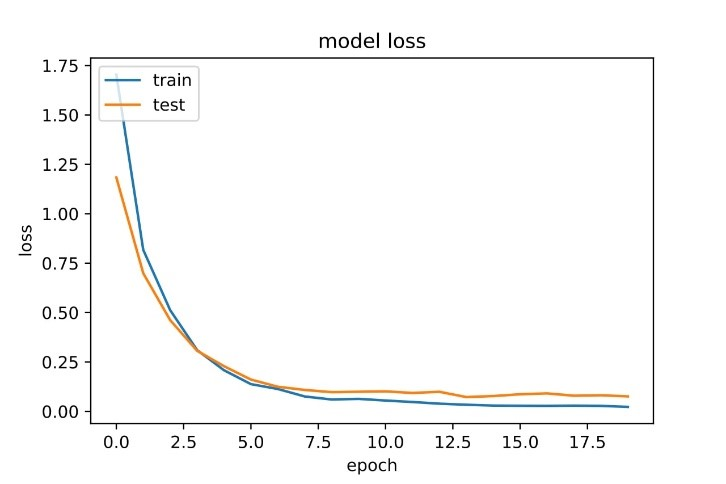
\includegraphics[width=\textwidth]{figures/Opt_RT/loss.jpg}
    \end{subfigure}
    
    \caption{\centering
    optimized models loss/accuracy in each epoch in real-time mode
    }
    \label{fig:org_rt}
\end{figure}








\begin{figure}
    \centering
    \begin{subfigure}[b]{0.2\textwidth}
        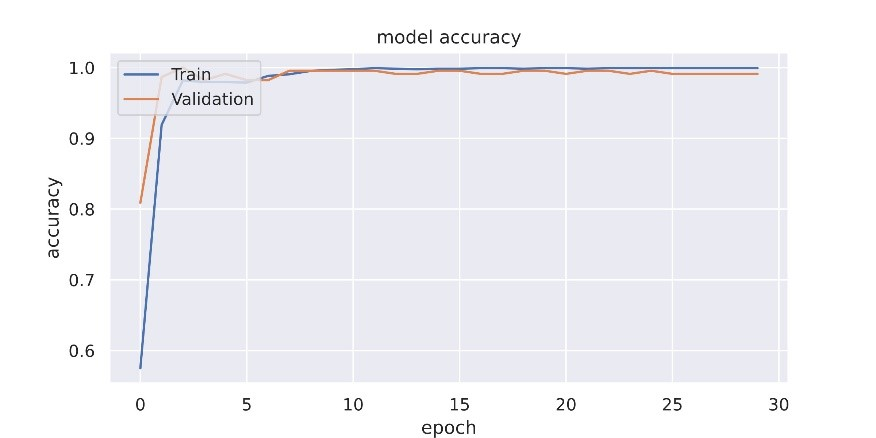
\includegraphics[width=\textwidth]{figures/Opt_OF/acc.jpg}
    \end{subfigure}
    \begin{subfigure}[b]{0.2\textwidth}
        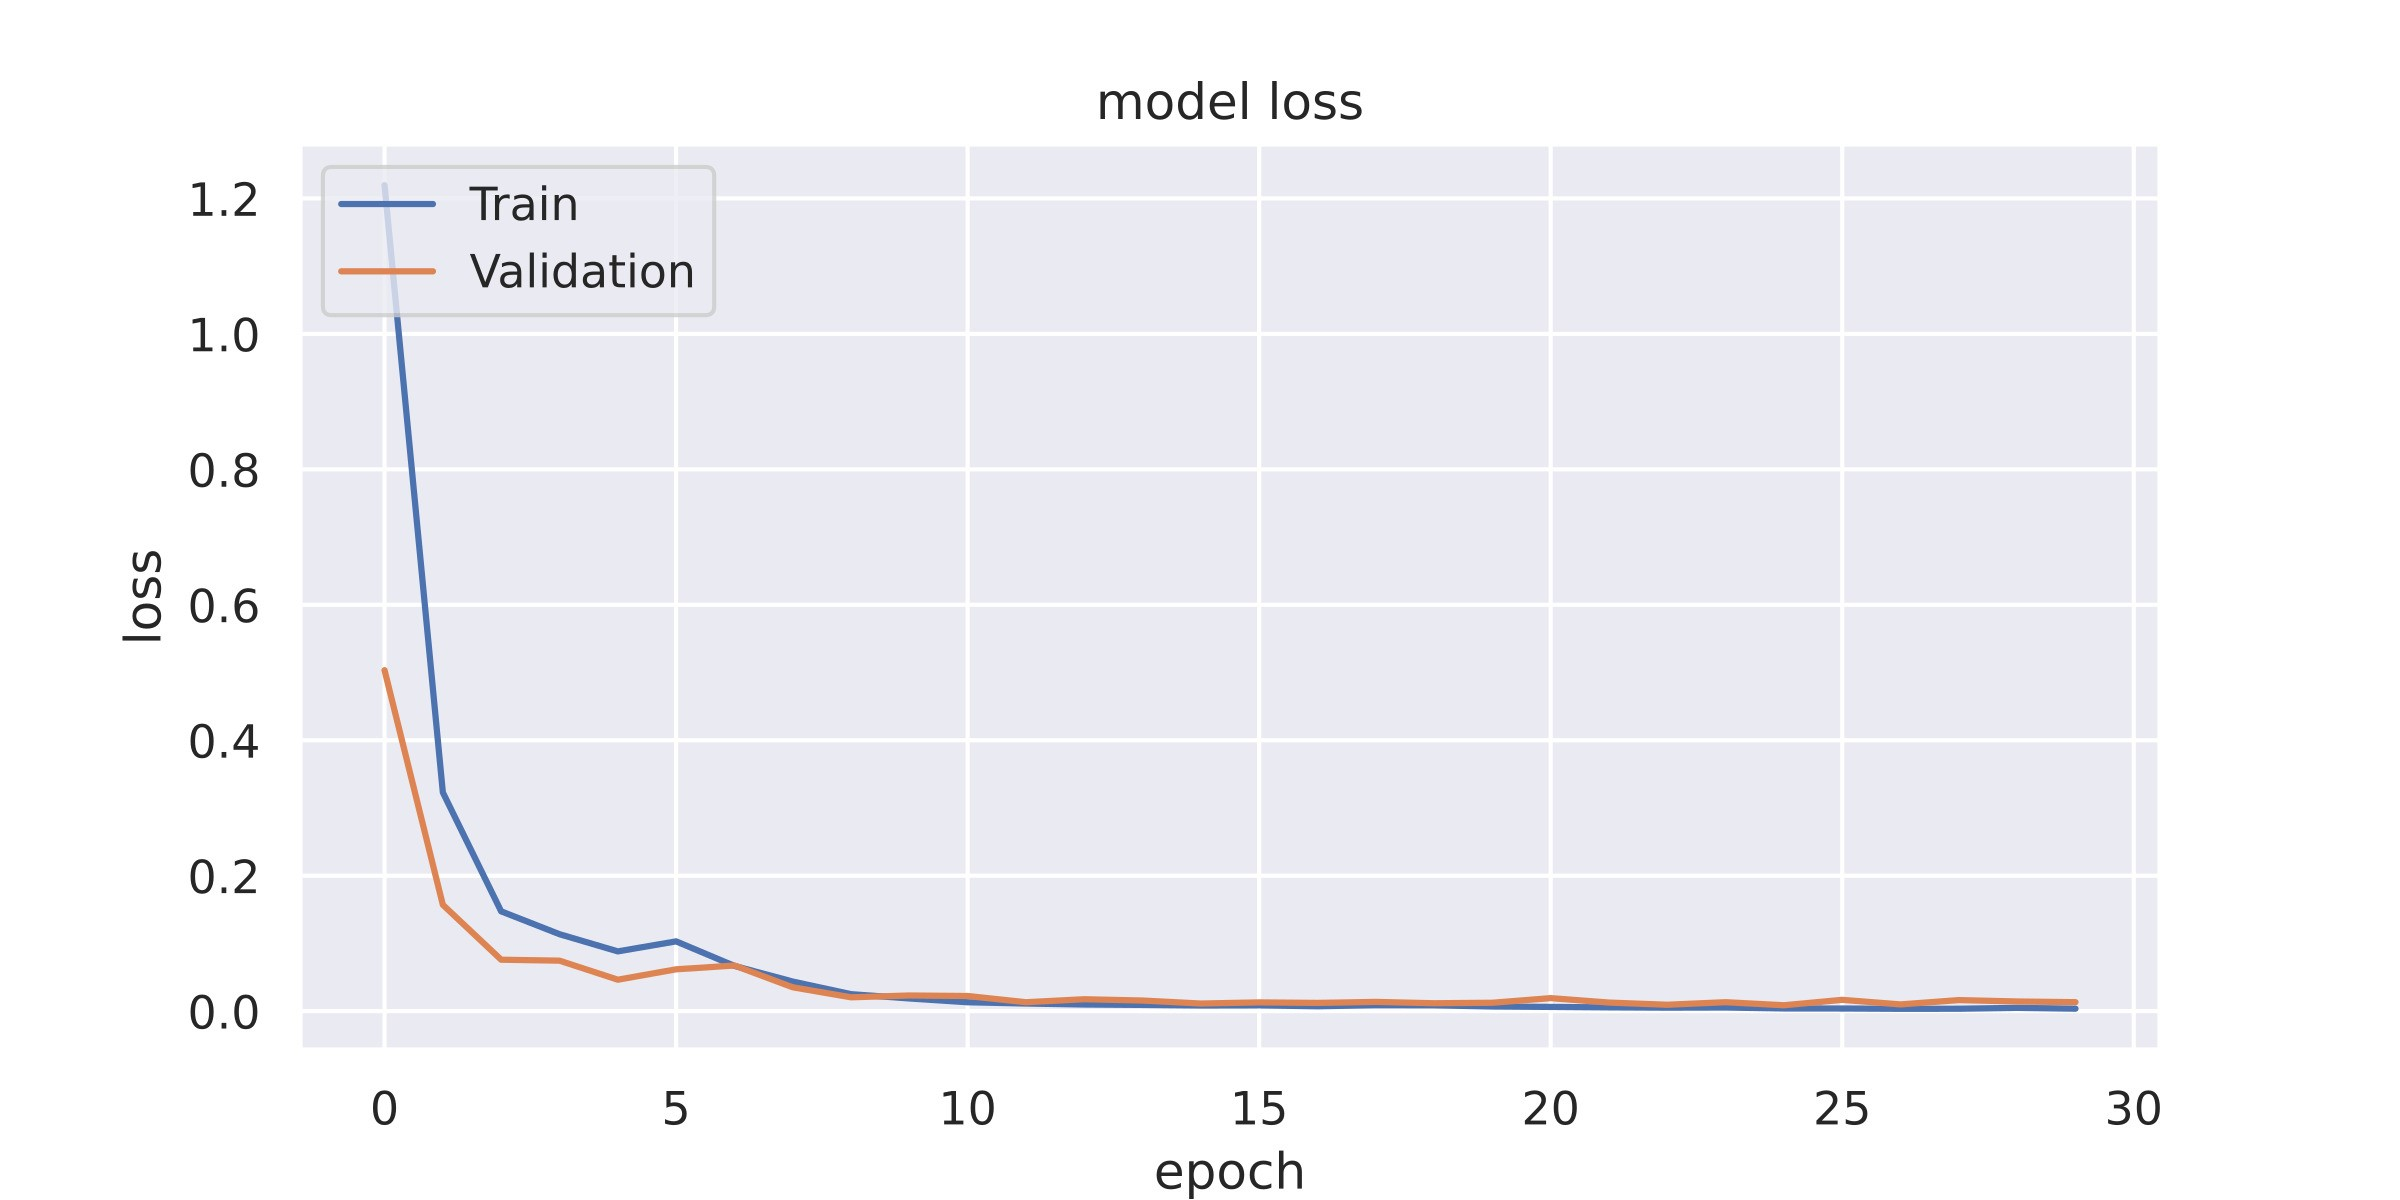
\includegraphics[width=\textwidth]{figures/Opt_OF/loss.jpg}
    \end{subfigure}
    
    \caption{\centering
    optimized models loss/accuracy  in each epoch in offline mode
    }
    \label{fig:org_of}
\end{figure}


% ================================================== %
% CONCLUSION
% ================================================== %
\section{conclusion}
In this study, a deep convolutional network optimized by a genetic algorithm was proposed to detect hand movements using forearm electromyographic signals. It was observed that although deep networks have a high potential in identifying the EMG patterns, they will not perform well unless their structure is appropriately arranged. In this work, only three parameters, the number of convolutional layers, the number of kernels in each convolutional layer, and the number of dense layer neurons, have been optimized. Finding the optimal value for these parameters increased the model accuracy from 91.86\% to 96.4\% at best, and 95.3\% on average in real-time usage. The accuracy of the optimized model in offline mode is 99.6\%. Optimizing the number of epochs and training the model up to 100\% convergence point can significantly affect the model's accuracy. The objective function of the genetic algorithm in this research is the accuracy of the model. To reduce the computational load, adding the number of independent model variables to the objective function's output can prevent the optimizer from moving toward larger models. In this case, a compromise is made between the accuracy of the model and the computational load. The authors focus on overcoming computational constraints and implementing new initiatives in model architecture and optimization in future work.






% trigger a \newpage just before the given reference
% number - used to balance the columns on the last page
% adjust value as needed - may need to be readjusted if
% the document is modified later
%\IEEEtriggeratref{8}
% The "triggered" command can be changed if desired:
%\IEEEtriggercmd{\enlargethispage{-5in}}

% references section

% can use a bibliography generated by BibTeX as a .bbl file
% BibTeX documentation can be easily obtained at:
% http://mirror.ctan.org/biblio/bibtex/contrib/doc/
% The IEEEtran BibTeX style support page is at:
% http://www.michaelshell.org/tex/ieeetran/bibtex/
%\bibliographystyle{IEEEtran}
% argument is your BibTeX string definitions and bibliography database(s)
%\bibliography{IEEEabrv,../bib/paper}
%
% <OR> manually copy in the resultant .bbl file
% set second argument of \begin to the number of references
% (used to reserve space for the reference number labels box)
\begin{thebibliography}{1}

\bibitem{IEEEhowto:kopka}
H.~Kopka and P.~W. Daly, \emph{A Guide to \LaTeX}, 3rd~ed.\hskip 1em plus
  0.5em minus 0.4em\relax Harlow, England: Addison-Wesley, 1999.

\end{thebibliography}

% You can push biographies down or up by placing
% a \vfill before or after them. The appropriate
% use of \vfill depends on what kind of text is
% on the last page and whether or not the columns
% are being equalized.

%\vfill

% Can be used to pull up biographies so that the bottom of the last one
% is flush with the other column.
%\enlargethispage{-5in}



% that's all folks
% \]
% \]
\end{document}